% Joshua Reed
% Fall, 2017
% 
% hw1.tex
% 
% Homework for introduction to probability.

\documentclass[12pt]{article}
\setlength\parindent{0pt}
 
\usepackage[margin=1in]{geometry} 
\usepackage{amsmath,amsthm,amssymb}
\usepackage{pgfplots}


\makeatletter
\renewcommand{\@seccntformat}[1]{}
\makeatother

% For Align:
%'*' tells LaTeX not to number lines.
%Align is a math environment. Thus \text{} is used for text contained within.
%'&' indicates a seperation between columns.

\begin{document}

{%Header section
  \large \bfseries 
  Joshua Reed \\
  Fall, 2017 \\
  \begin{center}
    {\huge Homework 1}\\
    MTH 361 - Introduction to Probability% chktex 8 
  \end{center}}
 
 
\section{1.7 \#3} 
\subsection{Exercise}
Two students pick a tire of four. What is the chance that they pick the same tire?

\subsection{Solution}
\subsubsection{Sample space for one student.}
The sample space is \{1,2,3,4\}. \\
Thus the chance that either picks any one tire is 1/4. 

\subsubsection{Sample space for one student then the other.}
The sample space is:
\begin{align*}
\Omega = \{&(1,1),(1,2),(1,3),(1,4),\\
           &(2,1),(2,2),(2,3),(2,4),\\
           &(3,1),(3,2),(3,3),(3,4),\\
           &(4,1),(4,2),(4,3),(4,4)\}
\end{align*}

\subsubsection{The event in which they pick the same tire.}
\begin{align*}
E = \{(1,1),(2,2),(3,3),(4,4)\}
\end{align*}

\subsubsection{Probability they pick the same tire.}
There are 4 ways to pick the same tire and 16 total ways to pick tires.

\begin{align*}
P(same) & = \frac{4}{16} \\
        & = \frac{1}{4}  
\end{align*}

\section{1.7 \#15} 
\subsection{Exercise} 
24\% have American Express cards, 61\% have visa, and 8\% have both. What percent have at least one credit card?

\subsection{Solution}
\subsubsection{Having at least one card is the union of those with either card.}
\begin{align*}
P(\geq \text{1 card}) & = P(AE) \cup P(V) \\
               & = P(AE) + P(V) - P(AE \cap V) \\
               & = 24\% + 61\% - 8\% \\
               & = 77%
\end{align*}

\section{1.7 \#25} 
\subsection{Exercise}
Alice attends 60\%, Betty attends 80\%. Their attendence is independent. What is the chance that at least one is there on 
a given day.
What is the chance that exactly one is there?

\subsection{Solution}
\subsubsection{Rule for the intersection of independent events.}
$P(A \cap B) = P(A)P(B)$
\subsubsection{Probability they both attend}

\begin{align*}
P(A \cap B) & = .6 * .8
            & = .48
\end{align*}

\subsubsection{Probability either attends is the probability of the union of the two events.}
\begin{align*}
P(A \cup B) & = P(A) + P(B) - P(A \cap B) \\
            & = .6 + .8 - .48 \\
            & = .92
\end{align*}

\subsubsection{The probability that exactly one attends.}
This is the probability that either attends minus the probability of both attending.
\begin{align*}
P(1) & = P(\geq 1)-P(A \cap B) \\
     & = .92-.48 \\
     & = .44
\end{align*}

\section{1.7 \#26}
\subsection{Exercise}
A and B are independent events
$P(A) = 0.4$
$P(A \cup B) = 0.64$
What is $P(B)$?

\subsection{Solution}
\subsubsection{Rule of independent events.}
$P(A \cap B) = P(A)P(B)$

\subsubsection{Probability of either events happening.}
$P(A \cup B) = P(A) + P(B) - P(A \cap B)$

\subsubsection{Relating the two above equations.}
$P(A \cup B) = P(A) + P(B) - P(A)P(B)$

\subsubsection{Solve}
\begin{align*}
0.64 & = 0.4 + P(B) - (0.4)P(B)
0.24 & = P(B) - (0.4)P(B)
0.24 & = (1 - 0.4)P(B)
0.24 & = (0.6)P(B)
P(B) & = \frac{0.24}{.6}
P(B) & = 0.4
\end{align*}

\subsubsection{The distribution of $|X-Y|$}
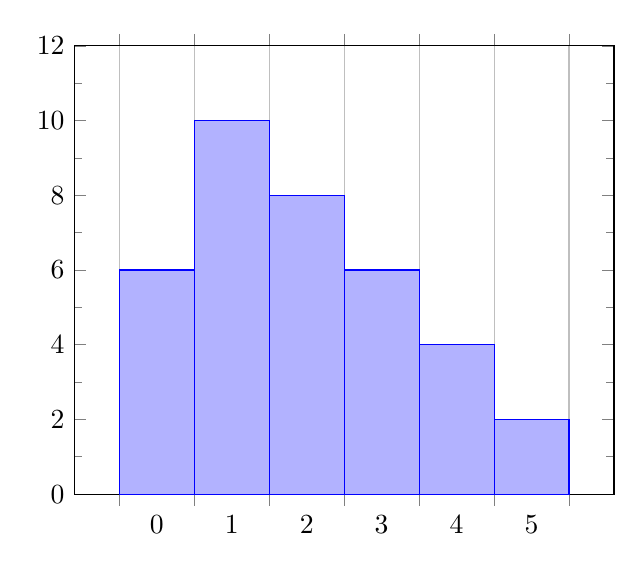
\begin{tikzpicture}
\begin{axis}[ybar interval, ymax=12,ymin=0, minor y tick num = 1]
\addplot coordinates {(0, 6) (1, 10) (2, 8) (3, 6) (4, 4) (5, 2) (6, 0)};
\end{axis}
\end{tikzpicture}
\end{document}










